\fontsize{13}{14}\selectfont
\chapter{Kết quả thực hiện}
\newpage
\section{Thi công mạch}
\subsection{PCB}
	\begin{figure}[H]
		\centering
		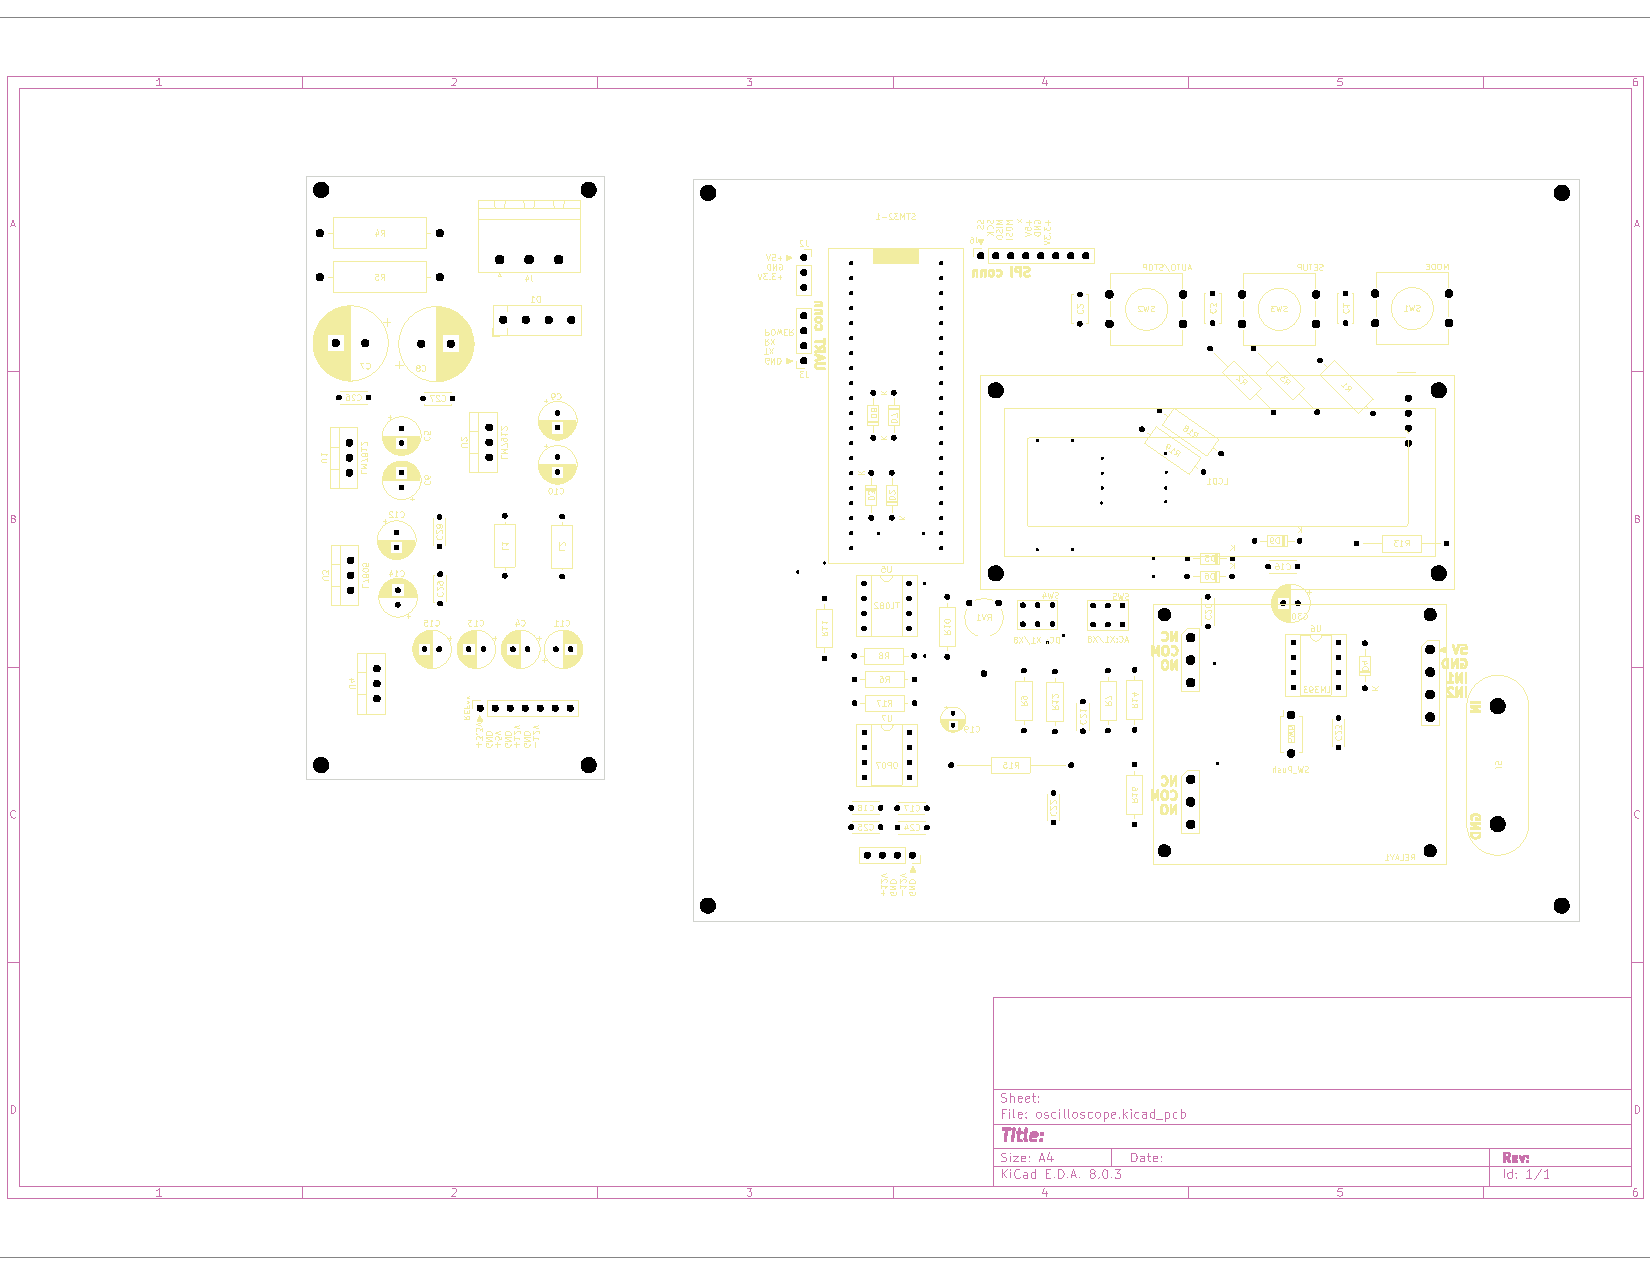
\includegraphics[width=0.8\linewidth]{./picture/layout_Fs.pdf}
		\caption{Lớp F.Silkscreen}
		\label{FSilkscreen}
	\end{figure}
	
	\begin{figure}[H]
		\centering
		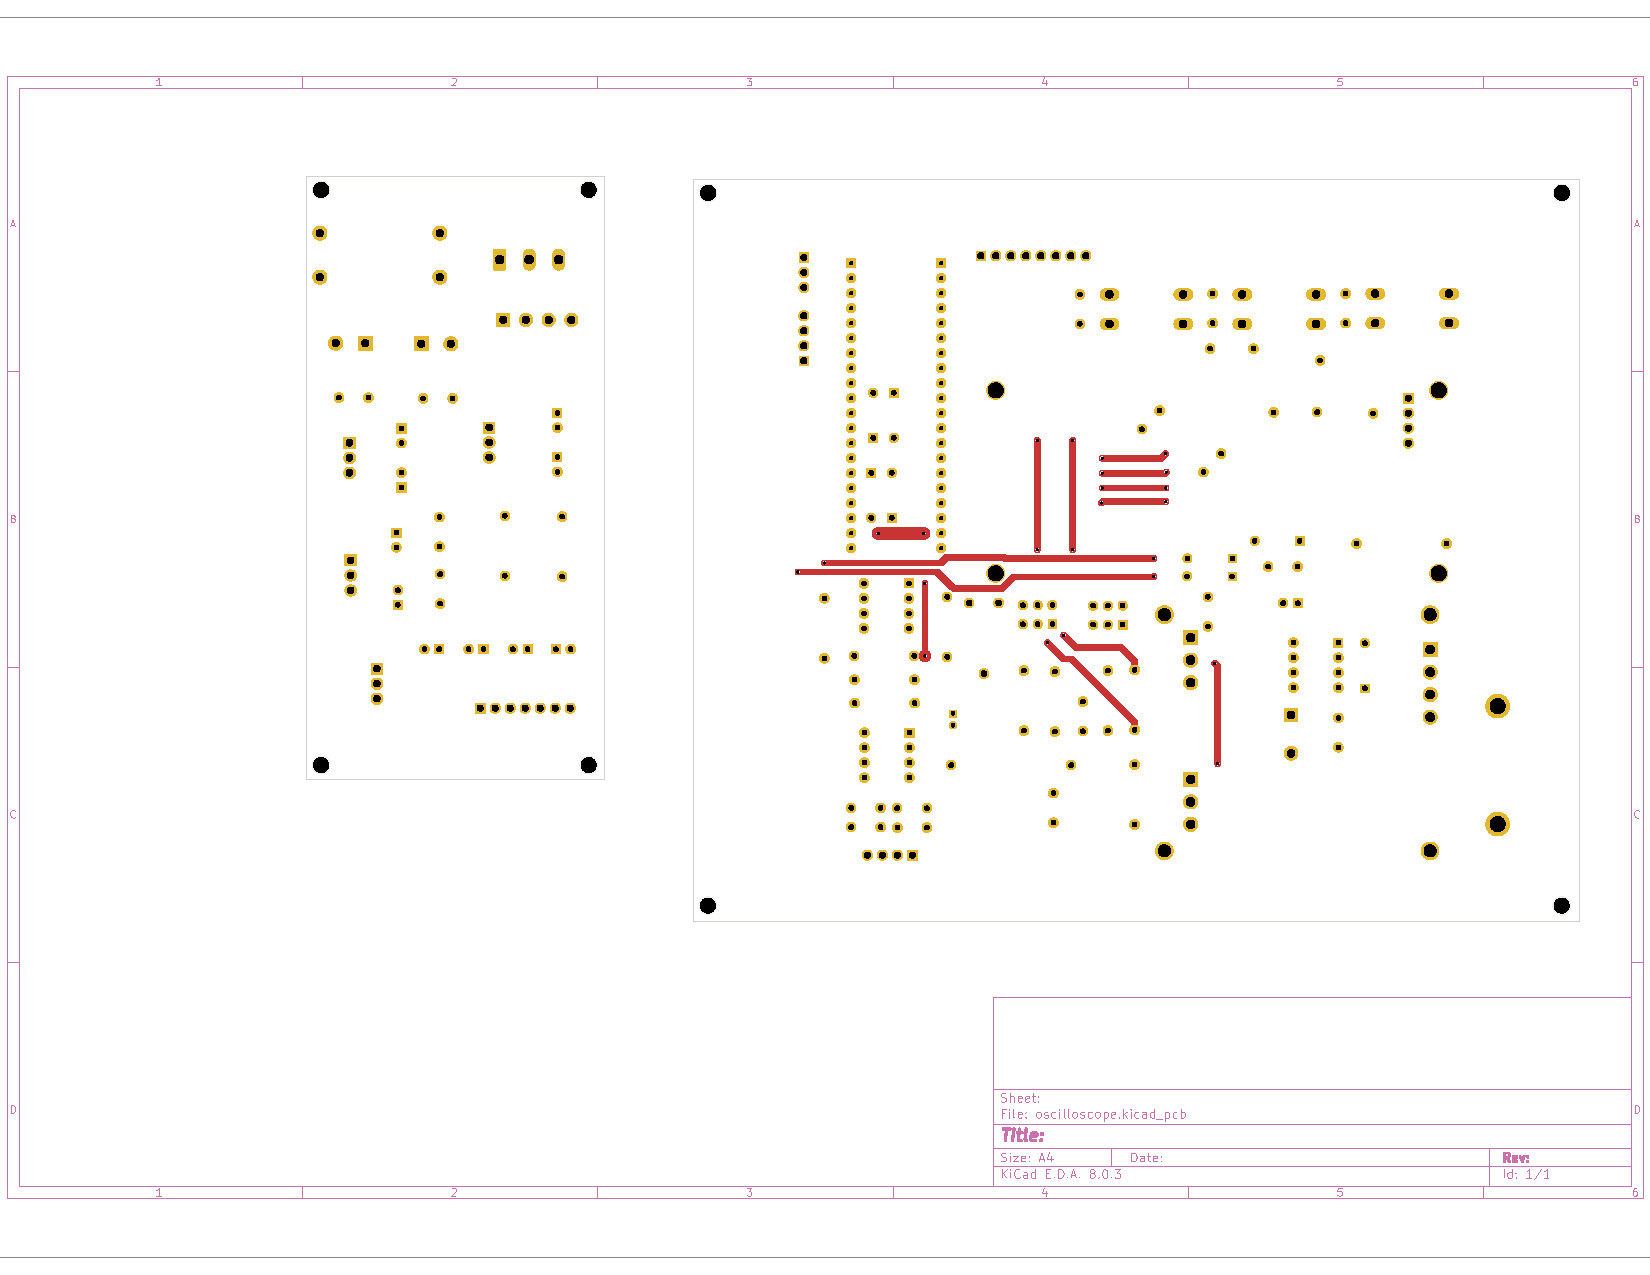
\includegraphics[width=0.8\linewidth]{./picture/layout_F.pdf}
		\caption{Lớp F.Cu}
		\label{Flayer}
	\end{figure}
	
	\begin{figure}[H]
		\centering
		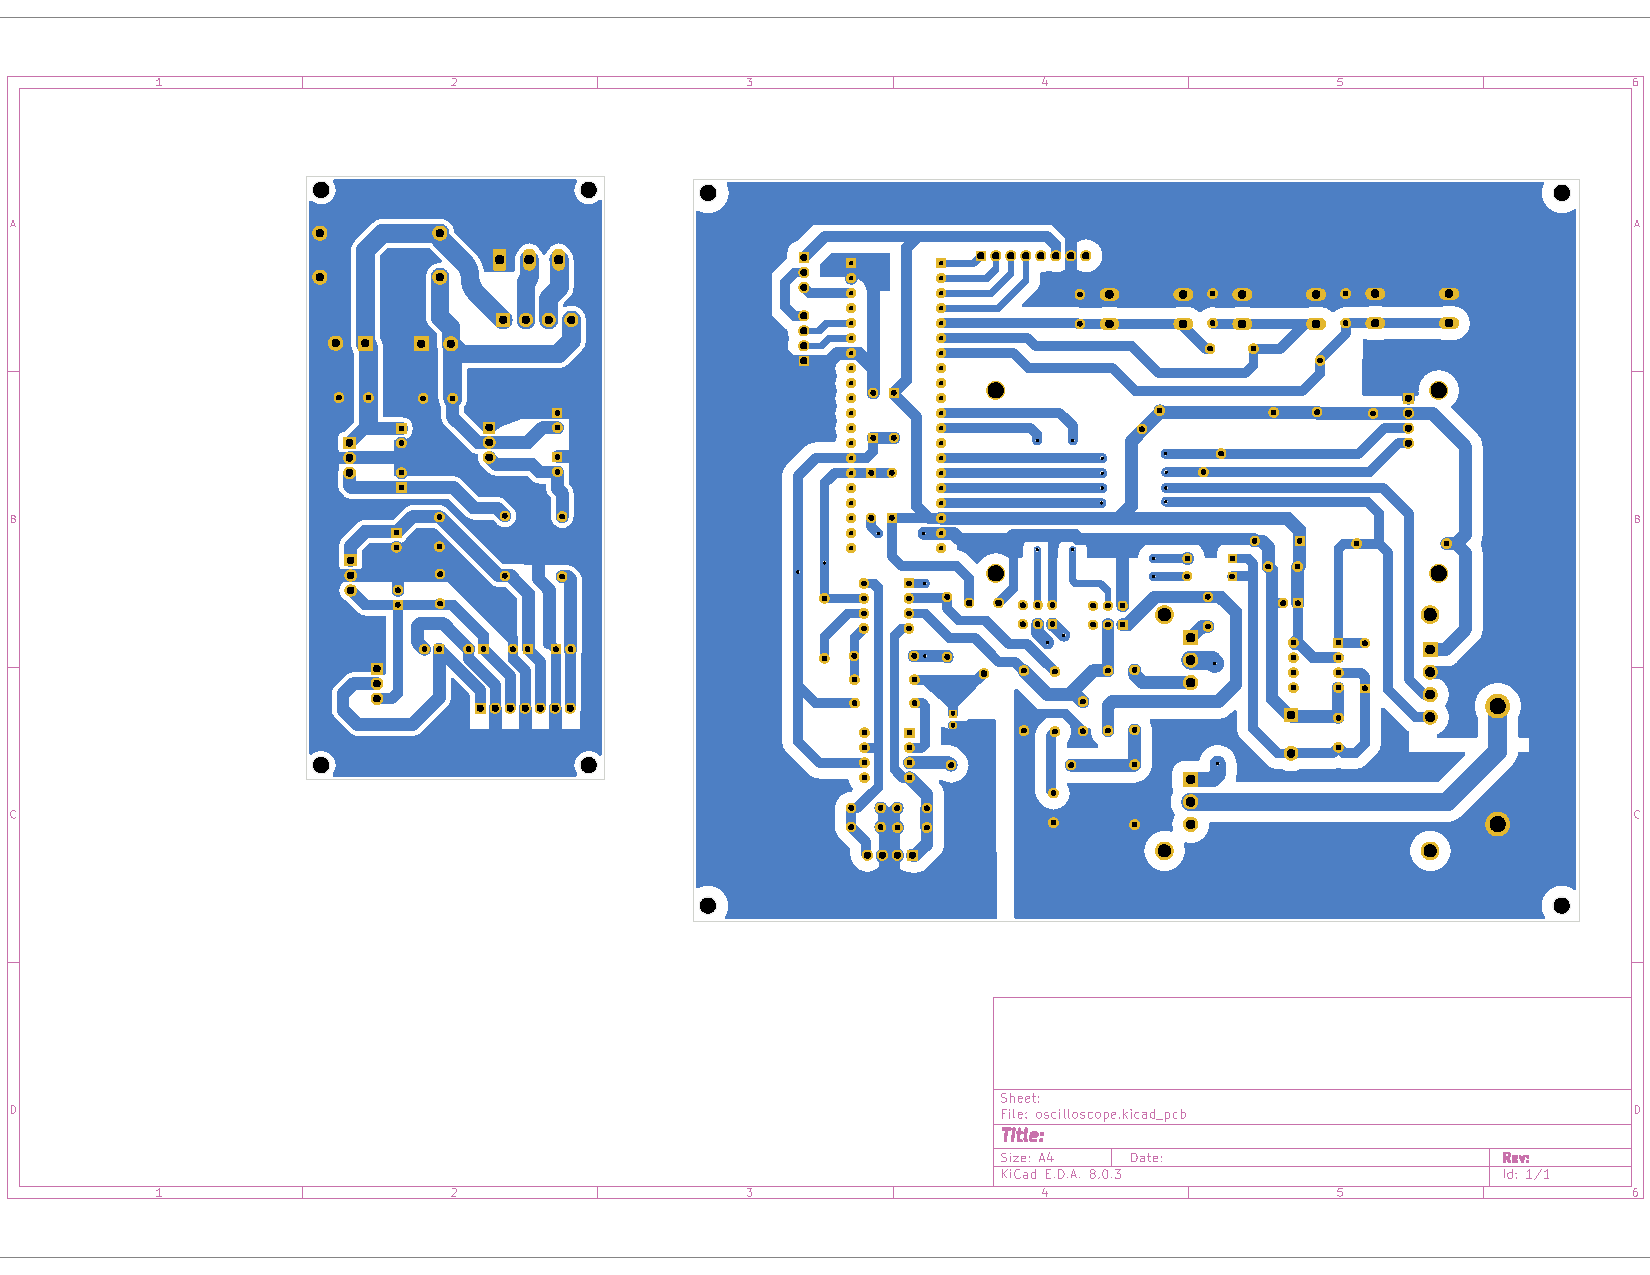
\includegraphics[width=0.8\linewidth]{./picture/layout_B.pdf}
		\caption{Lớp B.Cu}
		\label{Blayer}
	\end{figure}
	
	\begin{figure}[H]
		\centering
		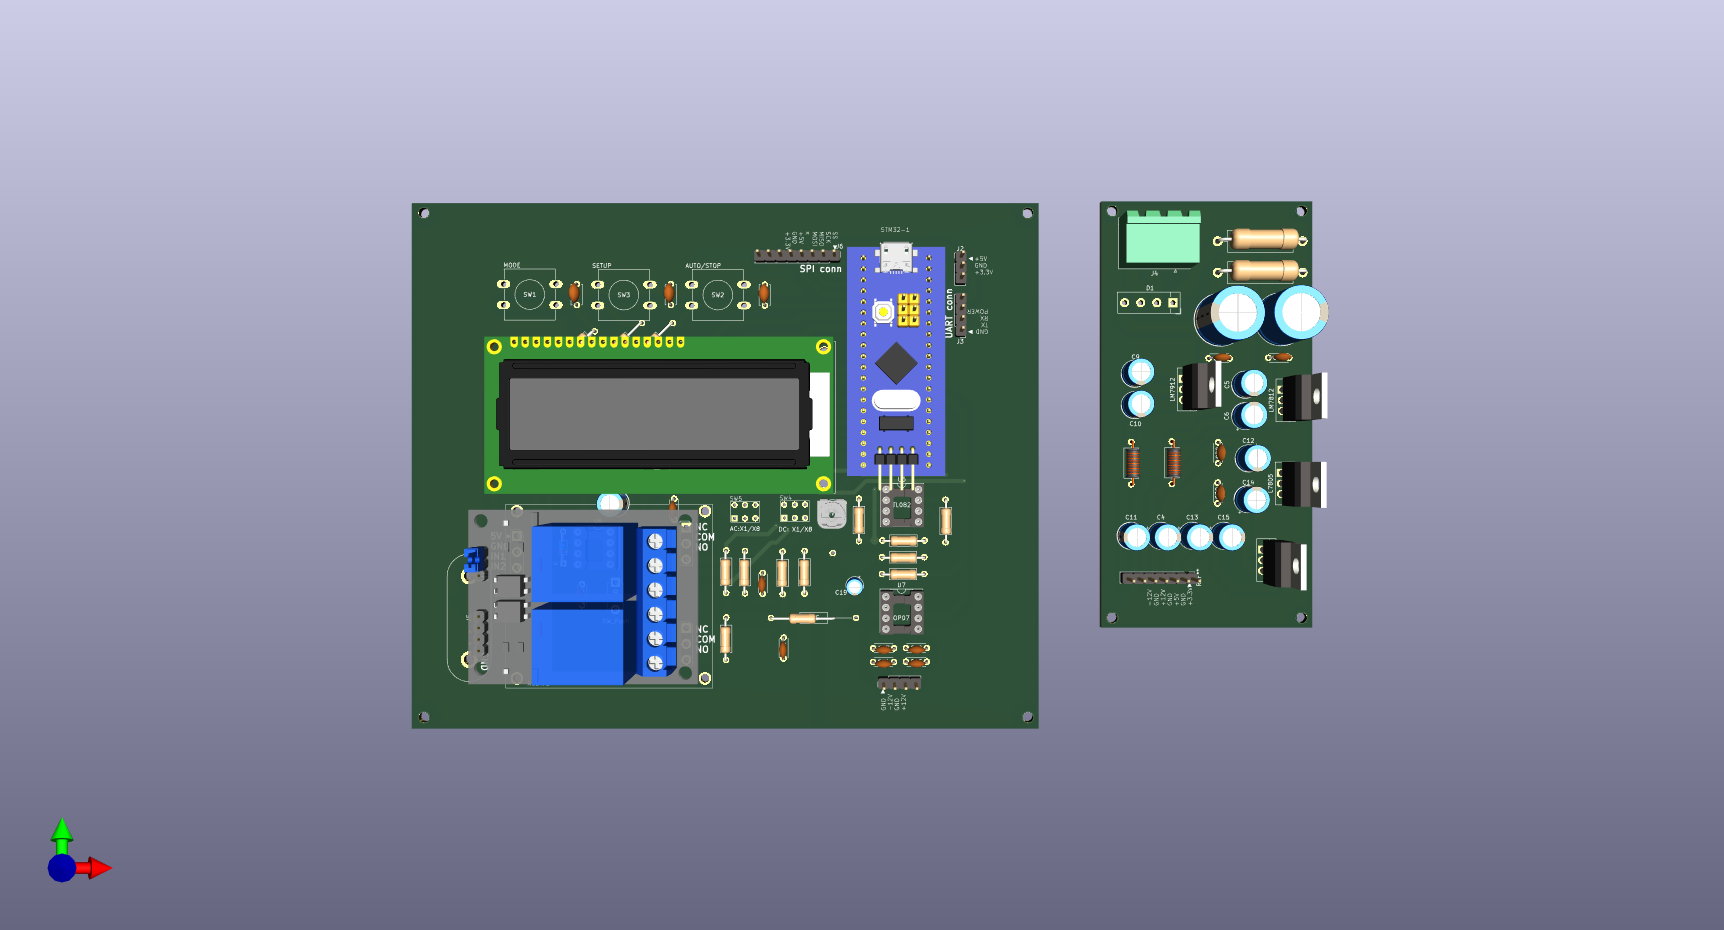
\includegraphics[width=0.8\linewidth]{./picture/model_3D.png}
		\caption{3D của hệ thống}
		\label{model 3D}
	\end{figure}
	
\subsection{Mạch thực tế}

	
		\begin{figure}[H]
			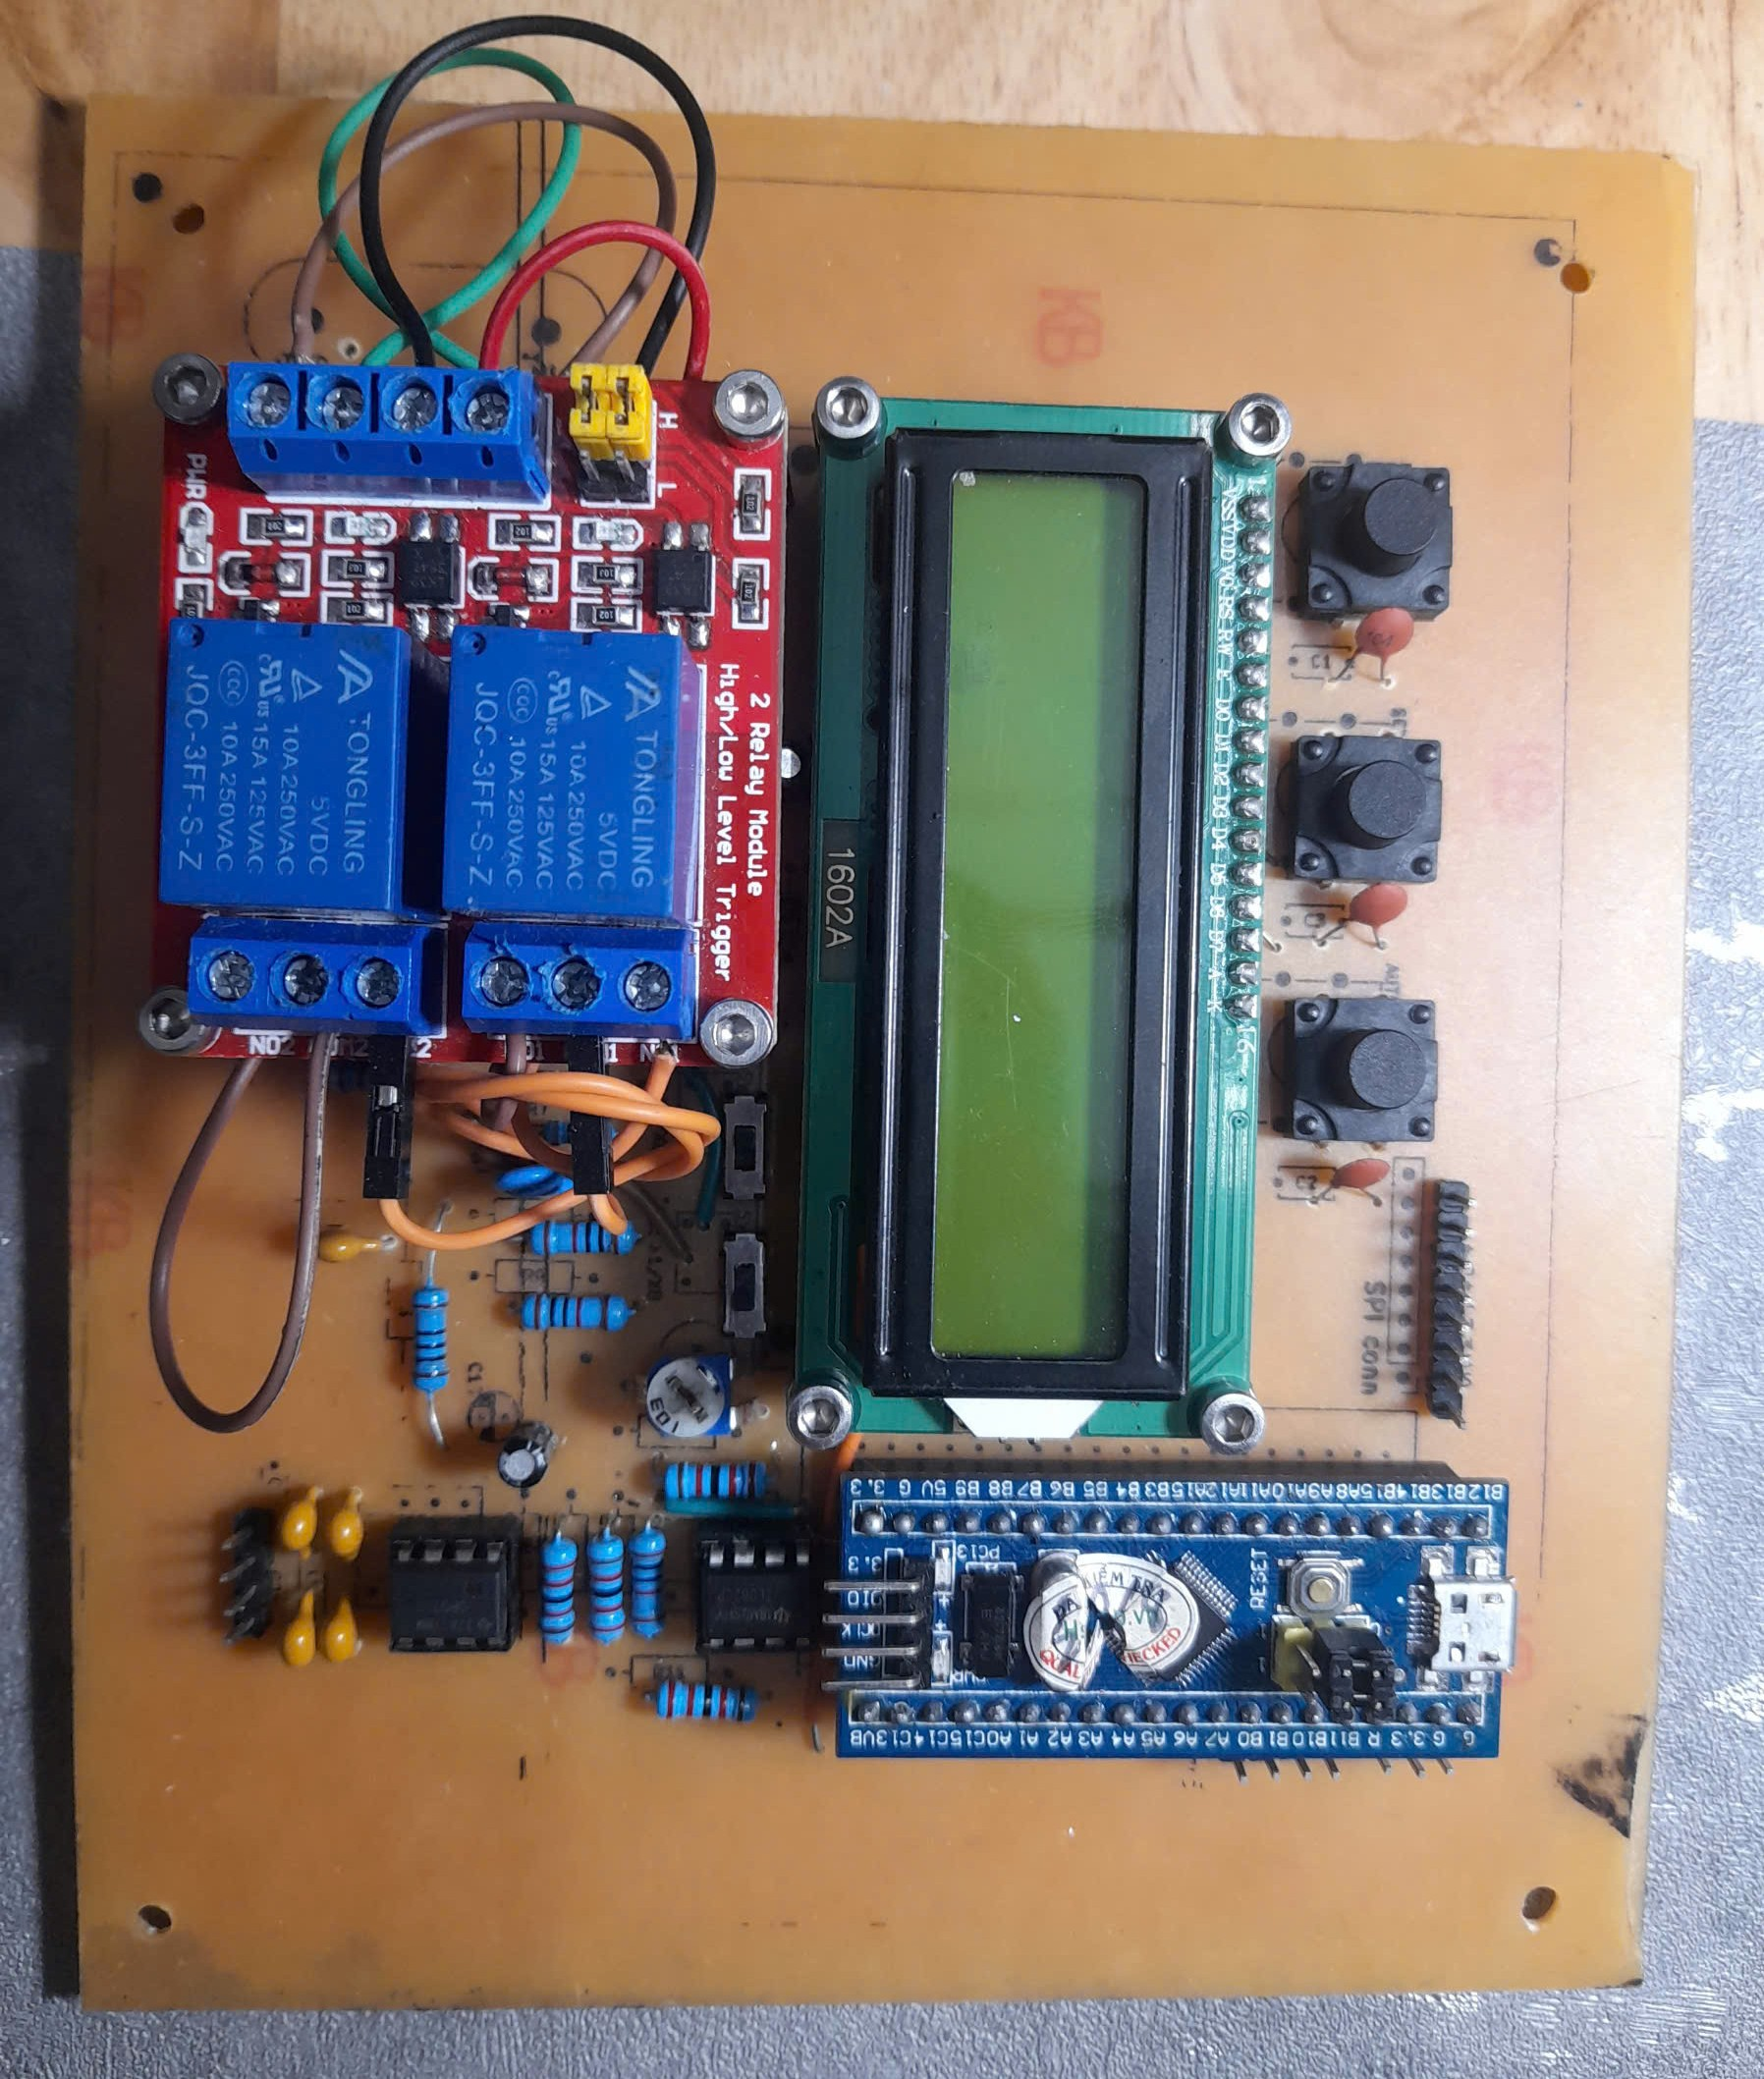
\includegraphics[width=\linewidth]{./picture/z6140688059060_129223f837543baa337e8804f1ab6d0e.jpg}
			\centering
			\caption{Mạch thực tế (phía trên)}
		\end{figure}
		
		\begin{figure}[H]
			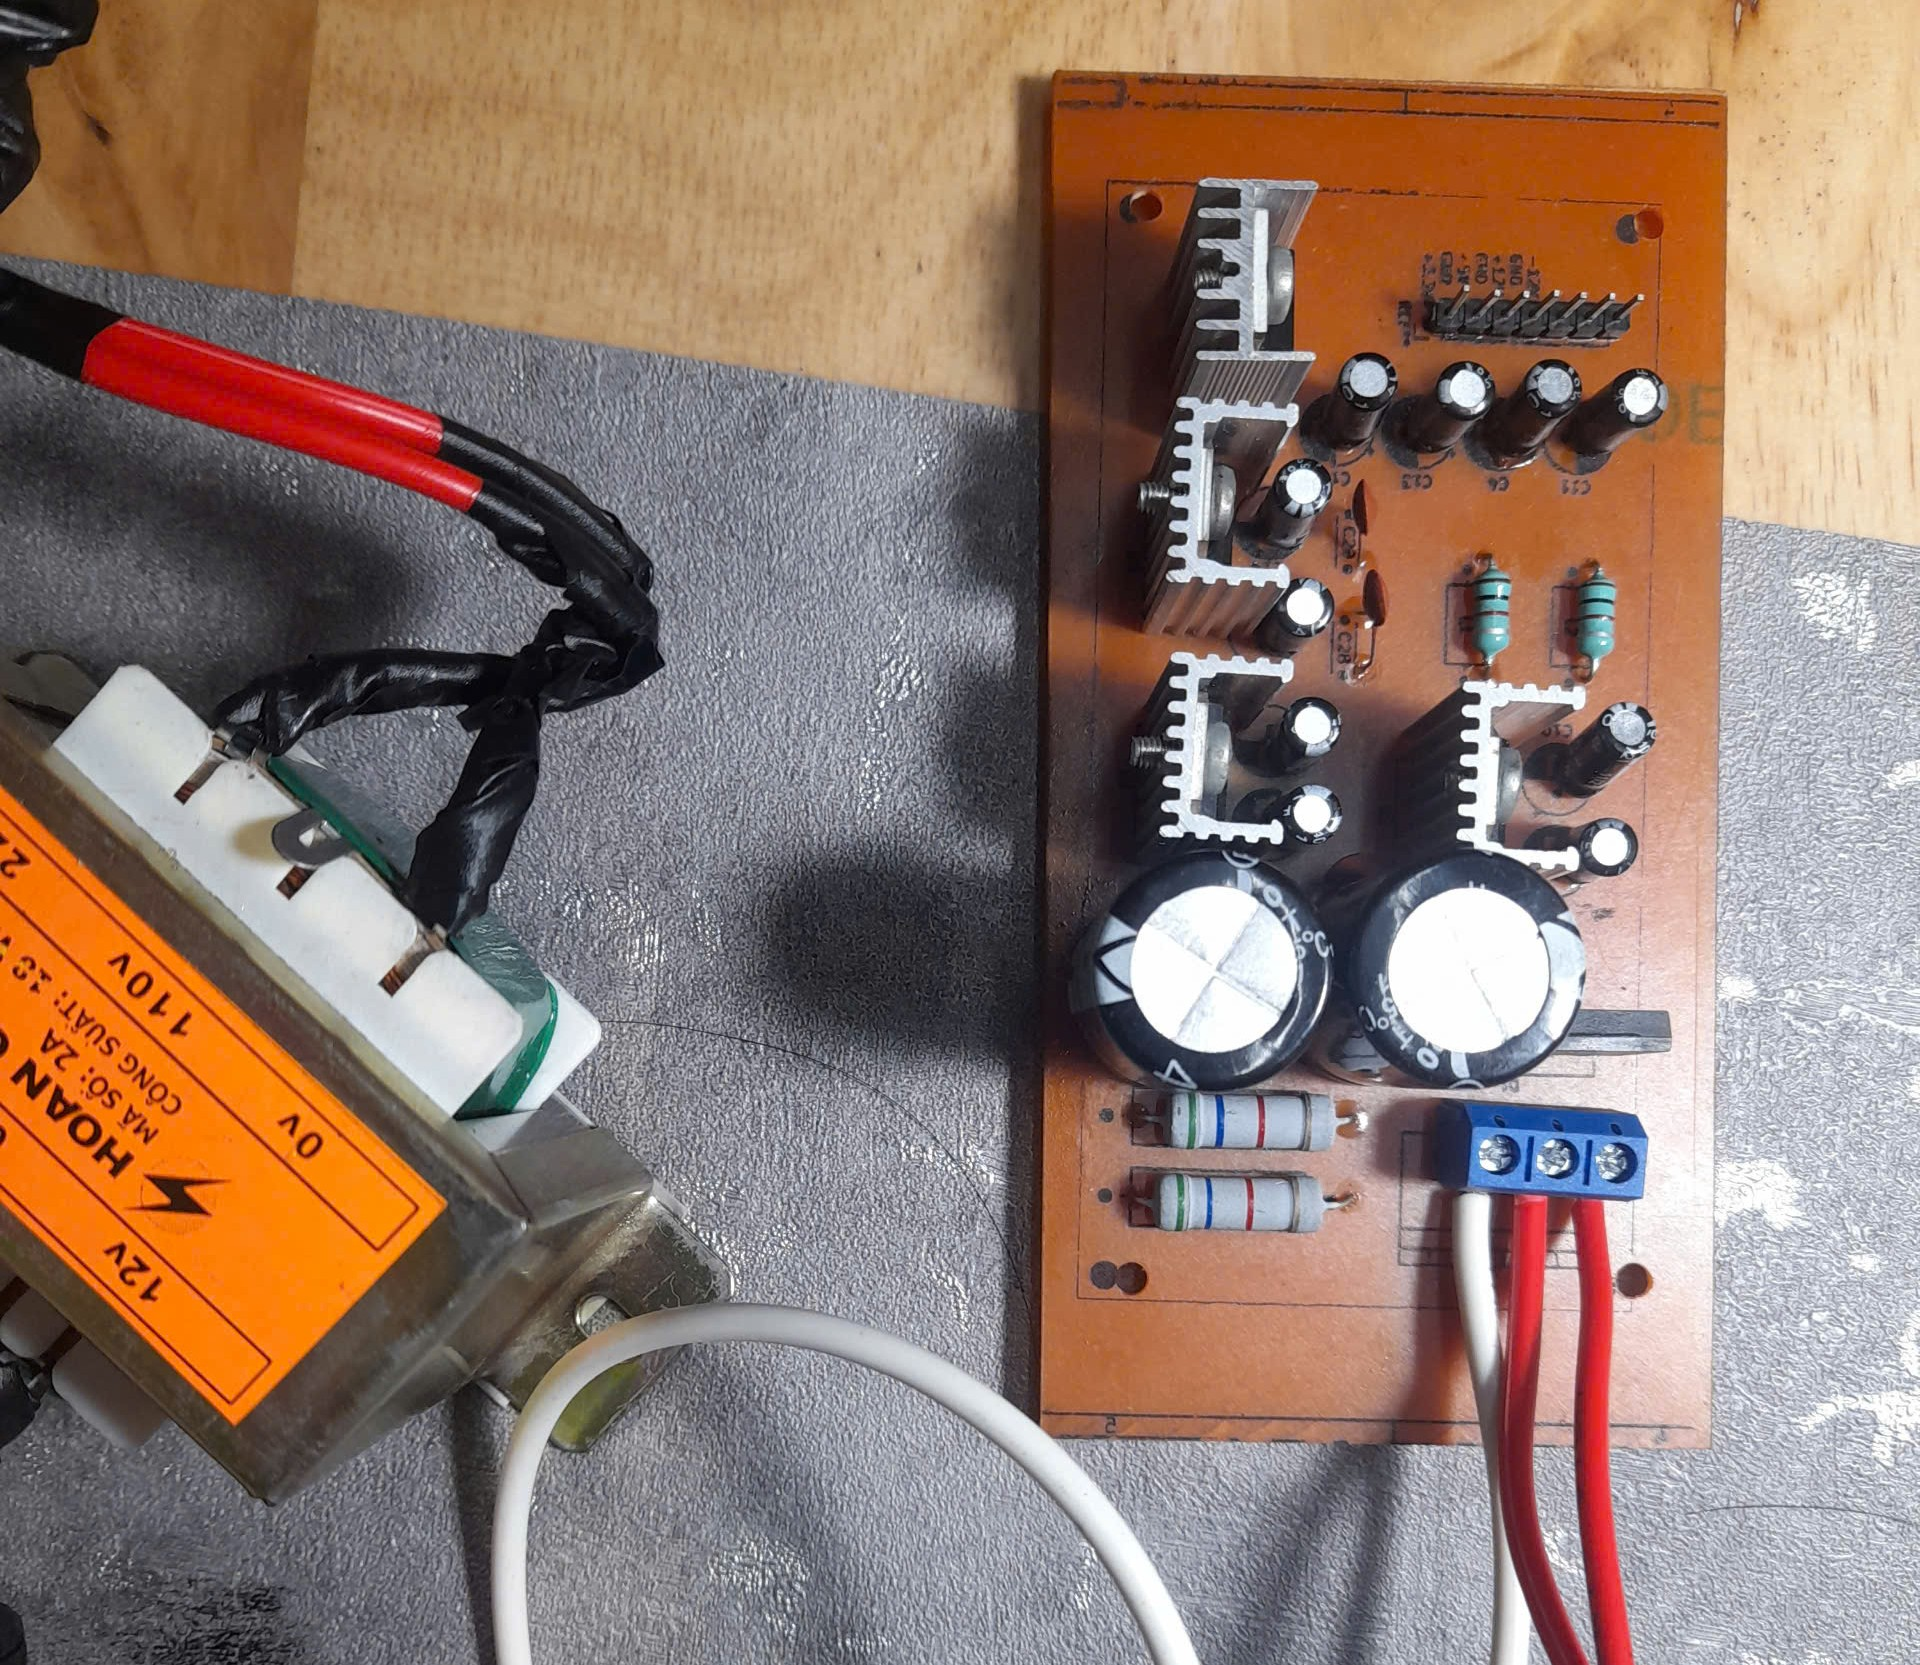
\includegraphics[width=\linewidth]{./picture/z6140688059187_549b6f11830970f120cc8764fab2aaa8.jpg}
			\centering
			\caption{Mạch thực tế (phía dưới)}
		\end{figure}
		
		\begin{figure}[H]
			\centering
			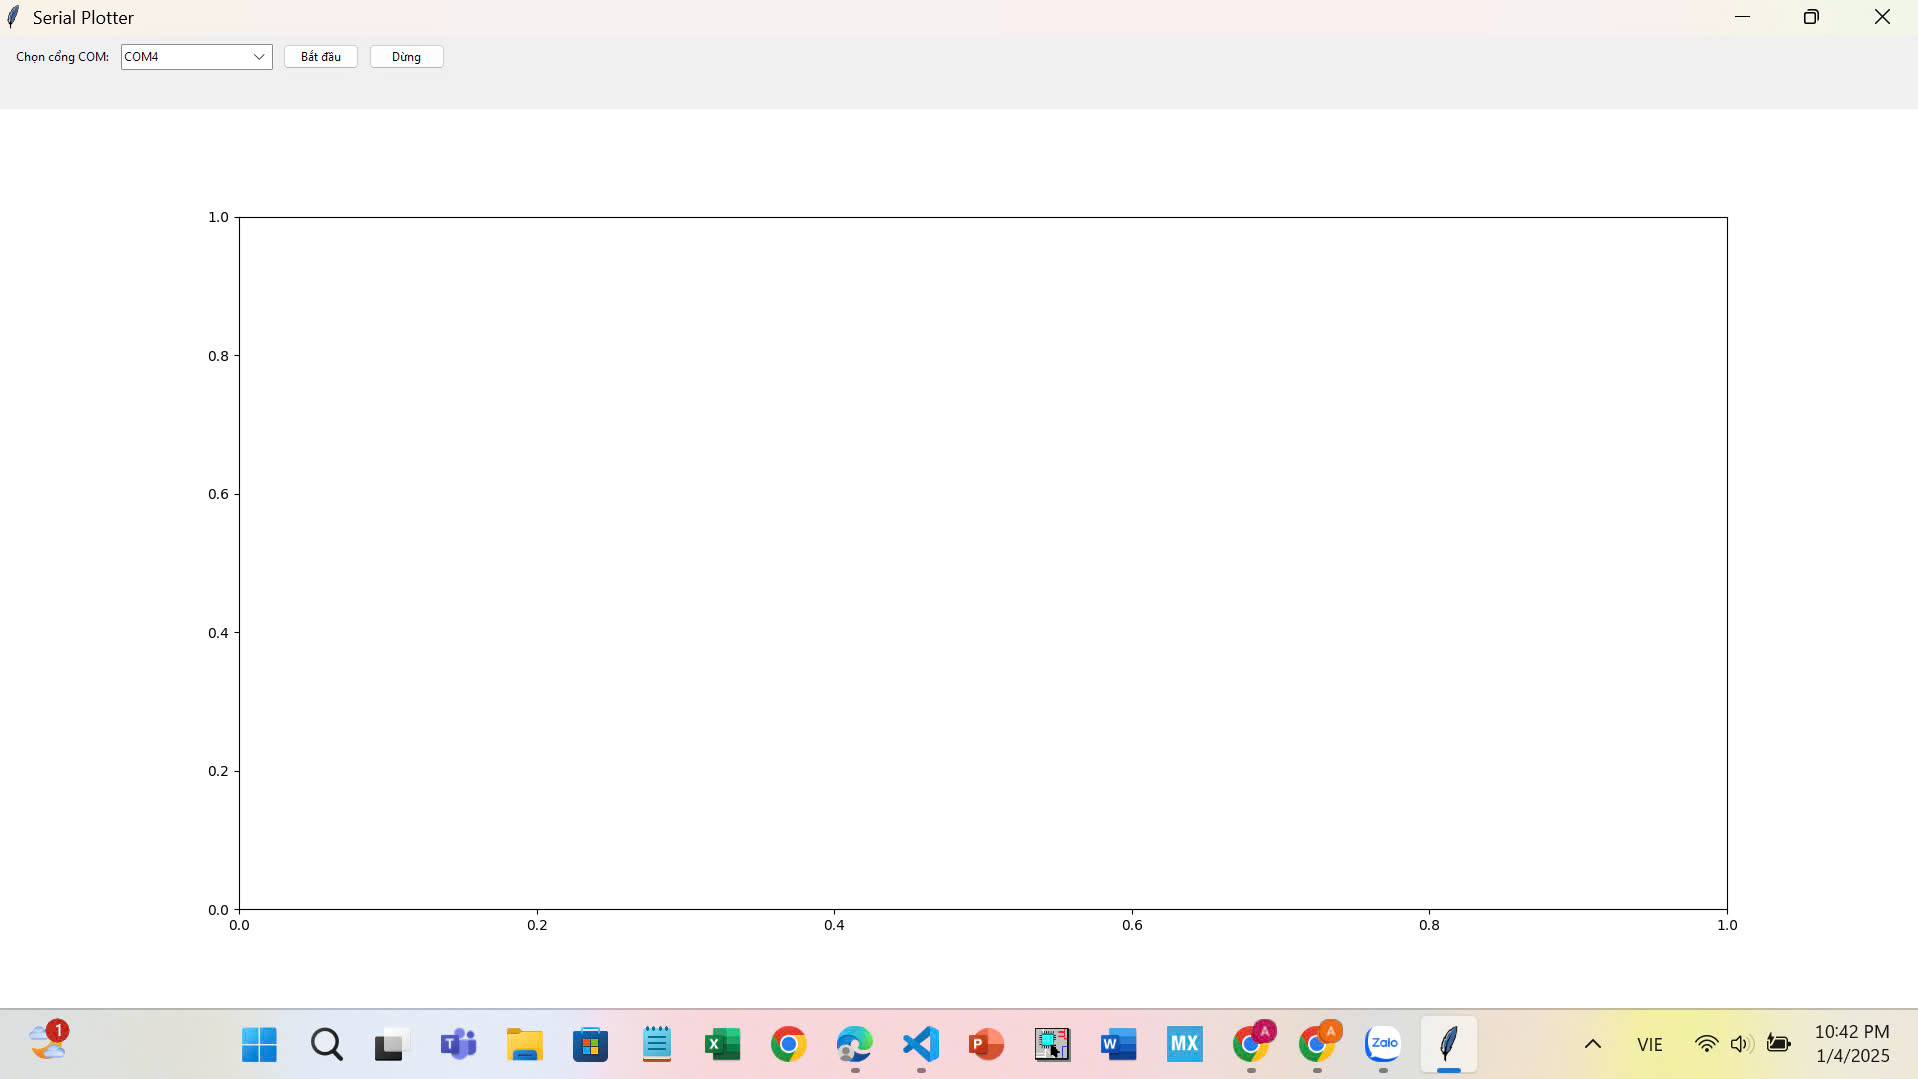
\includegraphics[width=\linewidth]{./picture/giao dien software.jpg}
			\caption{Giao diện hiển thị đồ thị}
		\end{figure}